\documentclass[11pt, a4paper, plain]{article}

\usepackage{fontspec}
\usepackage{inputenc}
\usepackage[czech]{babel}
\usepackage{luavlna}
\usepackage{graphicx}
\usepackage{tabularx}
\usepackage{array}
\usepackage[bookmarksopen,colorlinks,plainpages=false,linkcolor=black,urlcolor=blue,citecolor=black,filecolor=black,menucolor=black,unicode=true,breaklinks]{hyperref}
\usepackage{csquotes}
\usepackage{caption}
\usepackage{parskip}
\usepackage[margin=2.5cm, bindingoffset=1cm]{geometry}
\usepackage{titlesec}
\usepackage{lipsum}
\usepackage{todonotes}
\usepackage{csquotes}
\usepackage{latexcolors}
\usepackage{minted}
\usepackage{algorithm}
\usepackage{algpseudocode}
\usepackage{etoolbox}
\usepackage{amsmath}
\usepackage{booktabs}
\usepackage{colortbl}
\usepackage{siunitx}
\usepackage{svg}
\usepackage{tocloft}
\usepackage{bookmark}
\usepackage{subcaption}
\usepackage{enumitem}
\usepackage{amssymb}
\usepackage{unicode-math}
\usepackage{tabularx}
\usepackage{multirow}
\usepackage{hologo}

\setmainfont{Linux Biolinum G}
\setmonofont{Inconsolata}[Scale=0.925]
\setmathfont{Libertinus Math}

\setlength{\intextsep}{5mm} % nastavení mezery okolo obrázků
\setlength{\marginparwidth}{2cm}
\marginparsep=15pt
\linespread{1.3}
\unitlength=1mm % nastavení volby jednotek

% Use squares instead of circles
\setlist[itemize]{label = \raisebox{0.2ex}{\tiny$\blacksquare$}}

% Define not variants of if and while
\algnewcommand\algorithmicnot{\textbf{not}}
\algdef{SE}[IF]{IfNot}{EndIf}[1]{\algorithmicif\ \algorithmicnot\ #1\ \algorithmicthen}{\algorithmicend\ \algorithmicif}
\algdef{SE}[WHILE]{WhileNot}{EndWhile}[1]{\algorithmicwhile\ \algorithmicnot\ #1\ \algorithmicthen}{\algorithmicend\ \algorithmicwhile}

% Use default font for algorithmic
% \AtBeginEnvironment{algorithmic}{\rmfamily}

% Left-justified comment
\algnewcommand{\LeftComment}[1]{\Statex \(\triangleright\) #1}

% \usemintedstyle{tango}
\setminted{
    style=tango,
    bgcolor=ghostwhite,
    fontsize=\footnotesize,
    frame=none,
}

\AtBeginEnvironment{minted}{\linespread{0.3}}

% Use comma instead of period (czech standard)
\sisetup{locale = DE}

% List of attachments
\newcommand{\listappendixname}{Seznam příloh}
\newlistof{myappendices}{app}{\listappendixname}

% Tímto vypneš číslování stránek pouze pro tento seznam
\cftpagenumbersoff{myappendices}

% Příkaz pro přidání položky do seznamu příloh
\newcommand{\addextappendix}[1]{%
  \addcontentsline{app}{myappendices}{#1}
}

\begin{document}

\section*{Příloha G -- Popis vybraných periferií RP2350}

Tento dokument popisuje vybrané periferie RP2350: PWM, DMA a PIO.

\subsection{PWM v RP2350}

RP2350 obsahuje 12 generátorů PWM, v datasheetu odkazovaných jako \textit{PWM slice}. Každý slice
může řídit dva PWM výstupy, nebo měřit frekvenci nebo střídu vstupního signálu. Oba výstupy na
každém slicu mají stejnou periodu, ale nezávislé měnící střídu, takže ve výsledku máme 24
PWM výstupu.[14]

\begin{figure}[htbp]
    \centering
    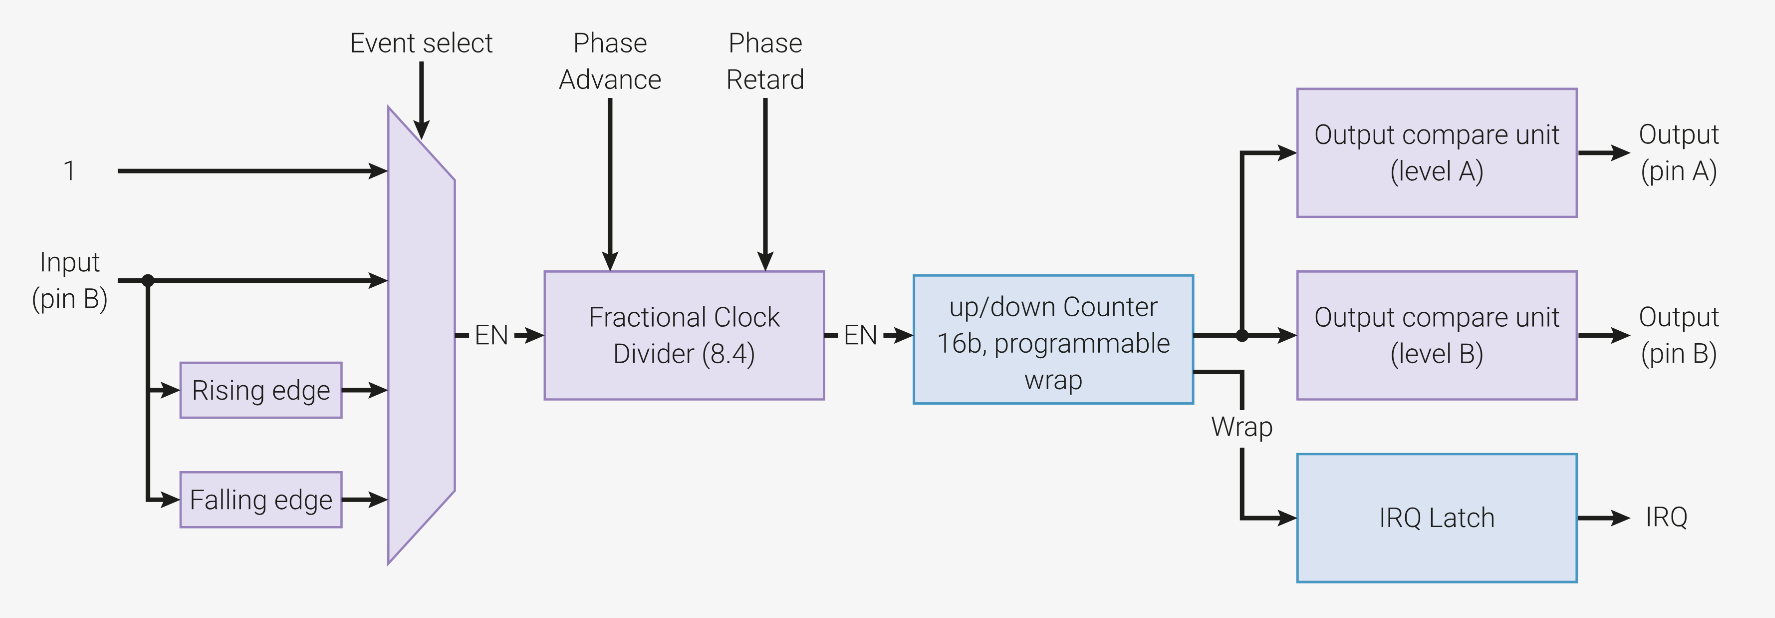
\includegraphics[width=\textwidth]{../../images/pwm_slice.png}
    \caption{Blokové schéma slicu PWM v RP2350. Zdroj [14].}
    \label{fig:pwm_slice}
\end{figure}

Každý PWM slice je vybaven 16bitovým vnitřním čítačem a 8.4 zlomkovým děličem hodin
(obr.~\ref{fig:pwm_slice}). Každý takt vnitřních hodin, slice nepřetržitě porovnává vstupní hodnotu
komparátoru s hodnotou vnitřního čítače, který se inkrementuje každý takt PWM. Když aktuální hodnota
je menší než vstupní hodnota, výstup PWM je logická 1. Jakmile hodnota čítače překoná vstupní
hodnotu, výstup se přepné na logickou 0. Vnitřní čítač se vynuluje když dosáhne TOP (nastavitelná
hodnota stropu) a cyklus se opakuje (obr. \ref{fig:rp2350_pwm}).

\begin{figure}[htbp]
    \centering
    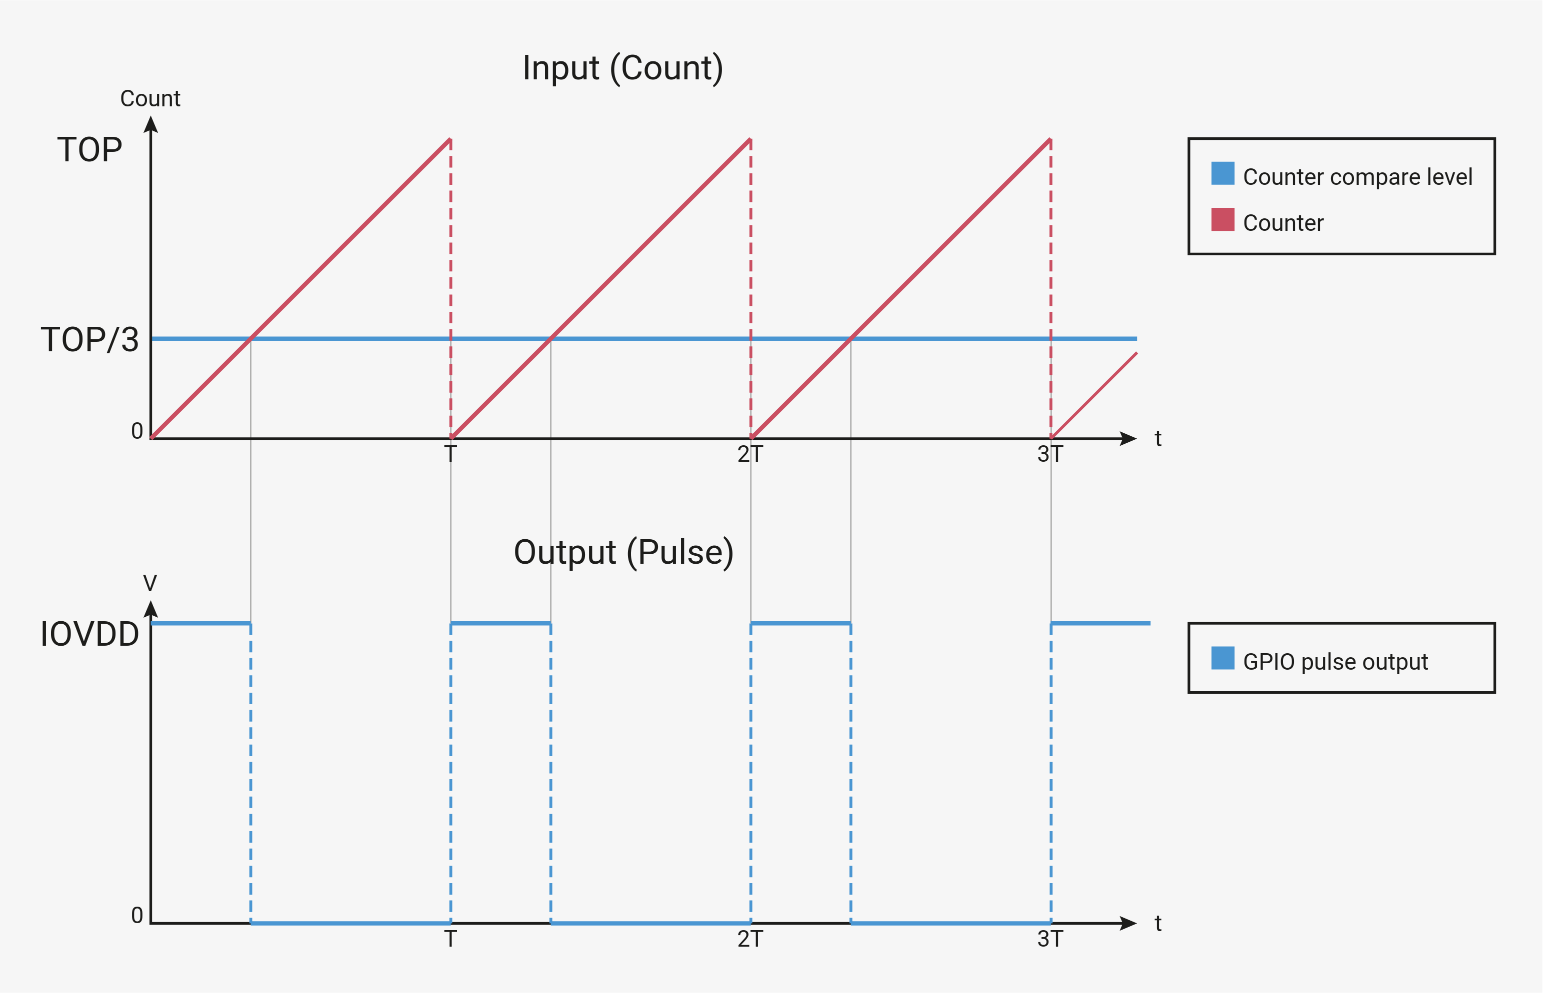
\includegraphics[width=\textwidth]{../../images/rp2350_pwm.png}
    \caption{Časový průběh PWM v RP2350. Zdroj [14].}
    \label{fig:rp2350_pwm}
\end{figure}

\subsection{DMA v RP2350}

RP2350 je vybaven 16 kanály DMA, každý z kterých ma konfigurovatelný zdroj, destinaci, rozměr
přenášených dat, dělič hodin atd. Každý DMA může nezávisle běžet, číst a zároveň zapisovat každý
cyklus.[14]

DMA může přenášet data v rámci RAM pamětí (\textit{memory-to-memory}), z RAM pamětí do periferie
(\textit{memory-to-peripheral}) nebo z periferie do RAM pamětí (\textit{peripheral-to-memory}).
Jedná z výhod tohoto je, že jeden DMA kanál může řídit jiný -- například spustit kanál, změnit adresu
čtení dat apod. To dovoluje implementovat složité a masivní přenosy dat, aniž by ovlivnilo činnost
mikrokontroléru.

\subsection{PIO v RP2350}

RP2350 je vybaven třemi bloky PIO, přičemž každý obsahuje čtyři nezávislé stavové automaty
(\textit{state machines}). Každý PIO blok představuje flexibilní hardwarové rozhraní, které dokáže
vykonávat vlastní zjednodušenou instrukční sadu nezávisle na hlavních procesorových jádrech. Každý
stavový automat má přístup k vyhrazeným FIFO frontám pro oboustranné předávání (RX a FIFO fronty)
dat mezi PIO a hlavním procesorem a dokáže s velkou přesností ovládat GPIO piny. Díky tomu je PIO
ideální pro implementaci vlastních nebo nestandardních sériových protokolů bez zátěže
procesoru.[14]

\begin{figure}[htbp]
    \centering
    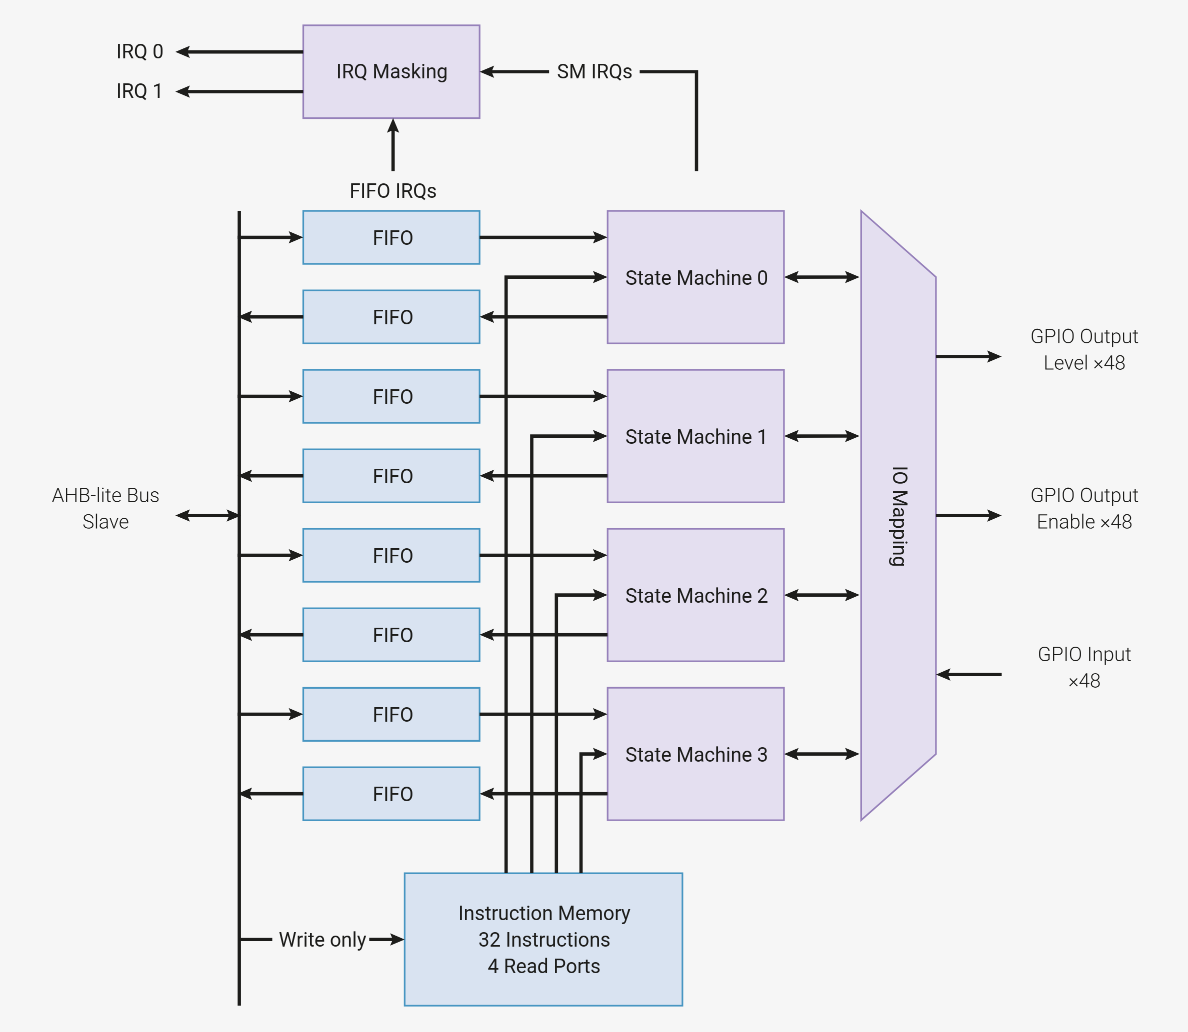
\includegraphics[width=\textwidth]{../../images/pio_block.png}
    \caption{Blokové schéma PIO bloku. Zdroj [14].}
    \label{fig:pio_block}
\end{figure}

Každý stavový automat disponuje vstupním posuvným registrem (ISR), výstupním posuvným registrem
(OSR) a pracovnými registry X a Y.

Programy pro PIO se píší ve specializovaném asembleru, který se pak překládá do strojového kódu
pomocí programu \textbf{pioasm}, který je součástí vývojové sady pico-sdk. PIO disponuje celkem
devíti instrukcemi, které jsou představeny v tabulce \ref{tab:pio_isa}.

\begin{table}
    \centering
    \begin{tabular}{llp{5cm}l}
        \toprule
        \textbf{Mnemotechnika} & \textbf{Popis} \\
        \midrule
        \texttt{JMP} & Skok na adresu, pokud podmínka je pravdivá. \\
        \texttt{WAIT} & Čekat dokud podmínka se nestane pravdivou.. \\
        \texttt{IN} & Posunout $N$ bitů ze zdroje do ISR. \\
        \texttt{OUT} & Posunout $N$ bitů z ISR do destinace. \\
        \texttt{PUSH} & Přesunout obsah ISR do RX FIFO. ISR bude vynulován \\
        \texttt{PULL} & Načíst 32bitové slovo z TX FIFO do OSR. \\
        \texttt{MOV} & Zkopírovat data ze zdroje do destinace. \\
        \texttt{IRQ} & Zapnout nebo vypnout příznak IRQ podle indexu. \\
        \texttt{SET} & Zapsat data do destinace. \\
        \bottomrule
    \end{tabular}
    \caption{Instrukční sada PIO.}
    \label{tab:pio_isa}
\end{table}

\end{document}
